\documentclass[11pt]{aghdpl}
% \documentclass[en,11pt]{aghdpl}  % praca w języku angielskim

% Lista wszystkich języków stanowiących języki pozycji bibliograficznych użytych w pracy.
% (Zgodnie z zasadami tworzenia bibliografii każda pozycja powinna zostać utworzona zgodnie z zasadami języka, w którym dana publikacja została napisana.)
\usepackage[english,polish]{babel}

% Użyj polskiego łamania wyrazów (zamiast domyślnego angielskiego).
\usepackage{polski}

\usepackage[utf8]{inputenc}

% dodatkowe pakiety

\usepackage{mathtools}
\usepackage{amsfonts}
\usepackage{amsmath}
\usepackage{amsthm}
%\usepackage{natbib}
\usepackage{gensymb}

% --- < bibliografia > ---

\usepackage[
style=numeric,
sorting=none,
%
% Zastosuj styl wpisu bibliograficznego właściwy językowi publikacji.
language=autobib,
autolang=other,
% Zapisuj datę dostępu do strony WWW w formacie RRRR-MM-DD.
urldate=iso8601,
% Nie dodawaj numerów stron, na których występuje cytowanie.
backref=false,
% Podawaj ISBN.
isbn=true,
% Nie podawaj URL-i, o ile nie jest to konieczne.
url=false,
%
% Ustawienia związane z polskimi normami dla bibliografii.
maxbibnames=3,
% Jeżeli używamy BibTeXa:
backend=biber
]{biblatex}

\usepackage{csquotes}
% Ponieważ `csquotes` nie posiada polskiego stylu, można skorzystać z mocno zbliżonego stylu chorwackiego.
\DeclareQuoteAlias{croatian}{polish}

\addbibresource{bibliografia.bib}

% Nie wyświetlaj wybranych pól.
%\AtEveryBibitem{\clearfield{note}}


% ------------------------
% --- < listingi > ---

% Użyj czcionki kroju Courier.
\usepackage{courier}

\usepackage{listings}
\lstloadlanguages{TeX}

\lstset{
	literate={ą}{{\k{a}}}1
           {ć}{{\'c}}1
           {ę}{{\k{e}}}1
           {ó}{{\'o}}1
           {ń}{{\'n}}1
           {ł}{{\l{}}}1
           {ś}{{\'s}}1
           {ź}{{\'z}}1
           {ż}{{\.z}}1
           {Ą}{{\k{A}}}1
           {Ć}{{\'C}}1
           {Ę}{{\k{E}}}1
           {Ó}{{\'O}}1
           {Ń}{{\'N}}1
           {Ł}{{\L{}}}1
           {Ś}{{\'S}}1
           {Ź}{{\'Z}}1
           {Ż}{{\.Z}}1,
	basicstyle=\footnotesize\ttfamily,
}

% ------------------------

\AtBeginDocument{
	\renewcommand{\tablename}{Tabela}
	\renewcommand{\figurename}{Rys.}
}

% ------------------------
% --- < tabele > ---

\usepackage{array}
\usepackage{tabularx}
\usepackage{multirow}
\usepackage{booktabs}
\usepackage{makecell}
\usepackage[flushleft]{threeparttable}

% defines the X column to use m (\parbox[c]) instead of p (`parbox[t]`)
\newcolumntype{C}[1]{>{\hsize=#1\hsize\centering\arraybackslash}X}


%---------------------------------------------------------------------------

\author{Bartosz Gil}
\shortauthor{B. Gil}

%\titlePL{Przygotowanie bardzo długiej i pasjonującej pracy dyplomowej w~systemie~\LaTeX}
%\titleEN{Preparation of a very long and fascinating bachelor or master thesis in \LaTeX}

\titlePL{Sprzętowo-programowy system wizyjny do detekcji pasa ruchu}
\titleEN{Hardware-software vision system for lane detection}


\shorttitlePL{Sprzętowo-programowy system wizyjny do detekcji pasa ruchu} % skrócona wersja tytułu jeśli jest bardzo długi
\shorttitleEN{Hardware-software vision system for lane detection}

\thesistype{Projekt dyplomowy}
%\thesistype{Master of Science Thesis}

\supervisor{dr inż. Tomasz Kryjak}
%\supervisor{Marcin Szpyrka PhD, DSc}

\degreeprogramme{Automatyka i Robotyka}
%\degreeprogramme{Computer Science}

\date{2019}

\department{Katedra Automatyki i Robotyki}
%\department{Department of Applied Computer Science}

\faculty{Wydział Elektrotechniki, Automatyki,\protect\\[-1mm] Informatyki i Inżynierii Biomedycznej}
%\faculty{Faculty of Electrical Engineering, Automatics, Computer Science and Biomedical Engineering}

\acknowledgements{Składam serdeczne podziękowania Panu Tomaszowi Kryjakowi za okazywaną cierpliwość i pomoc w trakcie przygotowywania pracy dyplomowej.}


\setlength{\cftsecnumwidth}{10mm}

%---------------------------------------------------------------------------
\setcounter{secnumdepth}{4}
\brokenpenalty=10000\relax

\begin{document}

\titlepages

% Ponowne zdefiniowanie stylu `plain`, aby usunąć numer strony z pierwszej strony spisu treści i poszczególnych rozdziałów.
\fancypagestyle{plain}
{
	% Usuń nagłówek i stopkę
	\fancyhf{}
	% Usuń linie.
	\renewcommand{\headrulewidth}{0pt}
	\renewcommand{\footrulewidth}{0pt}
}

\setcounter{tocdepth}{2}
\tableofcontents
\clearpage

\chapter{Wprowadzenie}

Samochód  autonomiczny jest to pojazd sterowany przez system komputerowy, w~oparciu o~dane z~wielu różnorodnych czujników. 
Według klasyfikacji SAE (ang. \textit{Society of Automotive Engineers} -- związek inżynierów zajmujących się motoryzacją) rozróżnia się pięć poziomów autonomizacji. 
Ostatni z~nich zakłada, że w sterowanie samochodu nie ma żadnej ingerencji ze strony człowieka. 
Pozostałe cztery odnoszą się do~różnego stopnia zaawansowania systemu ADAS (ang.\textit{Advanced Driving Assistance System} -- zaawansowany system wspomagania kierowcy).

Zadaniem systemów ADAS jest wspomaganie człowieka w czasie jazdy tj. wykrywanie i ostrzeganie o sytuacjach niebezpiecznych dla kierowcy i otoczenia. 
W~sytuacjach krytycznych komputer pokładowy jest w~stanie przejąć kontrolę nad autem i~wykonać manewr zapobiegający wypadkowi. 
Do postrzegania otoczenia wykorzystuje się czujniki takie jak radar, lidar, GPS, kamery, IMU (ang. \textit{inertial measurement unit}) oraz czujniki ultradźwiękowe.



Do podstawowych systemów ADAS zalicza się:
\begin{itemize}
	\item asystent parkowania - czujniki ultradźwiękowe rozmieszczone wokół samochodu umożliwiają mierzenie odległości pojazdu od innych przeszkód ułatwiając manewrowanie przy parkowaniu,
	\item monitorowanie martwego pola - kamery rozmieszczone bo bokach samochodu zbierają informacje z przestrzeni, których kierowca nie jest w stanie kontrolować wykorzystując z pomocy lusterek,
	\item ostrzeganie o kolizji przedniej, tylnej - tempomaty znajdujące się z przodu i z tyłu auta mierzą prędkość z jaką pojazd zbliża się do przeszkody. Gdy jest zbyt duża i istnieje ryzyko kolizji, system uruchomia alarm w postaci wizualnej lub dźwiękowej, a nawet dostosuje prędkość w celu uniknięcia kolizji,
	\item detekcja i rozpoznawanie znaków drogowych - system wykrywa i informuje kierowcę o znakach i~uruchamia sygnał alarmowy w przypadku niedostosowania się do nich,
	\item detekcja samochodów i pieszych - system przy pomocy kamer wykrywa ludzi i pojazdy znajdujące się w najbliższym otoczeniu oraz wyznacza ich przewidywaną ścieżkę ruchu. Jeśli istnieje ryzyko kolizji zostanie uruchomiony alarm. A w sytuacji krytycznej auto zahamuje,
	\item system ostrzegania przed opuszczeniem pasa ruchu (ang. \textit{Lane Departure Warning System}) -- jest to~mechanizm opierający się na detekcji linii drogowych i rozpoznawaniu jezdni. W~sytuacji, w~której samochód zaczyna zmieniać pas ruchu bez uprzednio włączonego odpowiedniego kierunkowskazu system wysyła ostrzeżenie do~kierowcy. Może to być sygnalizacja w postaci wizualnej, dźwiękowej lub wibracji. Wyróżnia się też bardziej zaawansowane wersje oprogramowania, w~których system przejmuje kontrolę nad układem kierowniczym i~nie pozwala na~zmianę pasa ruchu przez pojazd lub kieruje nim na środek pasa. Tego typu systemy zostały zaprojektowane w~celu zminimalizowania liczby wypadków drogowych wynikających z~błędów kierowców powodowanych między innymi przez zmęczenie bądź utrate koncentracji.
\end{itemize}

W ostatnim czasie można zauważyć spory rozwój w dziedzinie pojazdów bezzałogowych. Jest to~spowodowane widocznym rozwojem w dziedzinie sensoryki. oraz jednostek obliczeniowych w dziedzinie CPU (ang. \textit{Central Processing Units}) i GPGPU (ang. \textit{General Purpose computing on Graphics Processing Units}). Dodatkowo kolejny firmy motoryzacyjne starają się osiągać coraz to lepsze rozwiązania w celu wyróżnienia się na tle konkurencji i zdobycia większego rozgłosu. Na horyzoncie już widać pierwsze przymiarki do oficjalnego startu sezonu wyścigów samochodów autonomicznych Roborace \cite{roborace}. Przez długi czas wyścigi samochodowe były poligonem doświadczalnym dla nowych technologii, które następnie mogły trafić do samochodów drogowych. Aktualnie większość elektronicznych wspomagaczy kierowcy zostało zakazanych w Formule 1 i wpływ wyścigów uległ osłabieniu. Ale skoro w przyszłości mamy poruszać się pojazdami autonomicznymi, Roborace może pomóc w opracowywaniu nowej technologii takich pojazdów.

Jednym z możliwych rozwiązań efektywnego rozwoju oprogramowania są układy Zynq SoC. Dzięki możliwości ich reprogramowania są wygodnym zamiennikiem układów ASIC (ang. \textit{Application-Specific Integrated Circuit} - układ scalony specyficzny dla aplikacji) \cite{ASIC_zynq}. Rekonfigurowalność układu zapewnia szybszy i tańszy rozwój oprogramowania oraz pozwala na naprawę błędów w oprogramowaniu bez konieczności tworzenia nowego układu.
Firma Xilinx oferuje specjalistyczne układy z myślą o systemach ADAS. Urządzenia takie jak XA Zynq™-7000 SoCs idealnie nadają się do wysokich wymagań obliczeniowych zaawansowanych systemów wspomagania kierowcy (ADAS) \cite{xilinx}.


\section{Cele pracy}
W niniejszej pracy podjęto temat detekcji jezdni dla potrzeb pojazdów autonomicznych.  
Celem pracy jest napisanie modelu programowego w~języku Matlab algorytmów przetwarzających nagrany obraz. 
Rezultatem powinien być film, na który naniesione są krzywe reprezentujące detekcje linii drogowych.
Kolejną częścią pracy jest przeprowadzenie implementacji sprzętowej algorytmów na układzie Zynq SoC(ang. \textit{System On Chip}) przy użyciu języka opisu sprzętu Verilog. 
\section{Układ pracy}
W rozdziale drugim przedstawiono przegląd metod przetwarzania obrazu wykorzystywanych w systemach ADAD. 
W~kolejnym rozdziale omówiono platformę Zybo Zynq SoC. 
Rozdział czwarty odnosi się do implementacji programowej. Natomiast w rodziale piątym poruszona zostaje kwesta implementacji sprzętowej. Szósty rozdział zawiera opis przeprowadzonych testów. Pracę kończy podsumowanie.
\chapter{Przegląd algorytmów z literatury}

\section{Wstępne przetwarzanie obrazu}
Pierwszym etapem detekcji pasów ruchu drogowego jest konwersja obrazu kolorowego w~formacie RGB (ang. \textit{Red, Green, Blue} -- czerwony, zielony, niebieski) na~obraz binarny.
Proces ten ma na celu aby wstępnie otrzymać cechy określające dany obraz oraz ułatwić dalsze jego przetwarzanie. W celu ułatwienia konwersji z kolorowego na binarny, możemy przekonwertować wstępnie obraz do formatu w skali szarości. 

Każdy piksel w~formacie RGB składa się z trzech kanałów, każdy przyjmuje wartośći z~przedziału od 0 do 255, gdzie 0 oznacza brak nasycenia danego koloru, a 255 maksymalne nasycenie.
W skali szarości na jeden piksel przypada tylko jeden kanał przyjmujący wartości od 0 do 255.
Dla obrazu binarnego na jeden piksel również przypada tylko jeden kanał, ale może przyjmowac wartości o lub 1, gdzie 0 to brak nasycenia kolorów, a 1 to pełne nasycenie kolorów.
Obraz w skali szarości z obrazu w~formacie RGB można otrzymać, np. wyznaczająć średnią wartość trzech kanałów dla każdego z pikseli \cite{4}, lub poprzez wykorzystanie składowej L z formatu HSL (ang. \textit{Hue, Saturation, Lightness} -- odcień, saturacja, jasność) \cite{reichenbach_comparison}.


Jednym z metod konwersji obrazu ze skali szarości do binarnego, który zaproponowano w~pracy \cite{4}, jest zwiększenie kontrastu dzięki wykorzystaniu rozciągania histogramu. Następnie korzystając z filtru Sobel'a uwydatnia się krawędzie obiektów, które ma na celu ułatwienie późniejszej detekcji linii pasa ruchu drogowego. Kolejno wykorzystuje się progowanie polegające na przypisywaniu wartości 0 lub 1 do piksela w zależności od tego czy jego wartość jest mniejsza od wartości progu, czy nie. Operator Sobel'a jest zasadniczo operatorem różniczkowania dyskretnego, zwraca pochodne pierunkowe obrazu w ośmiu kierunkach co 45 stopni \cite{3}, \cite{sobel}.


Innym podejściem \cite{reichenbach_comparison} jest wykorzystanie algorytmu Canny Edge Detector w miejscu filtra Sobel'a. Canny Edge łączy w sobie filtr sobela i zdefiniowaną histerezę \cite{cany}. Jeśli wartośc gradientu $G$ \eqref{eq:1} piksela jest powyżej ustalonego progu górnego, zaliczany jest do zbioru krawędzi. Gdy jest poniżej ustalonego progu dolnego piksel jest odrzucany. Gdy znajduje się pomiędzy oboma wspomnianymi progami, piksel zostanie zaliczony do zbioru krawędzi jeśli sąsiaduje z pikselem zaklasyfikowanym jako krawędź.

\begin{equation}
G_{x} = \begin{bmatrix} -1 & 0 & +1 \\ -2 & 0 & +2 \\ -1 & 0 & +1 \end{bmatrix}, G_{y} = \begin{bmatrix} -1 & -2 & -1 \\ 0 & 0 & 0 \\ +1 & +2 & +1 \end{bmatrix},
G = \sqrt{ G_{x}^{2} + G_{y}^{2} } \label{eq:1}
\end{equation}

Próg binaryzacji można również dobrać samodzielnie, np. przyjmując, że jego wartość jest równa połowie wartości maksymalnej jaką może mieć piksel \cite{1}. Innym podejściem, zaprezentowanym w~artykule \cite{2}, jest wykorzystanie funkcji entropii lub histogramu.
Histogram obrazu jest sposobem reprezentacji rozkładu wartości piksleli, z~których składa się obraz. 
Może przyjmować formę interpolowanego wykresu, gdzie pozioma oś układu współrzędnych odpowiada za wartość piksela. 
A pionowa oś reprezentuje liczebność punktów o~wartości równej wartości argumentu znajdującego się na~poziomej osi \cite{histogram}.
Na rysunku \ref{fig:entr_hist} przedstawiono zestawienie wykresu danego histogramu oraz wykresu funkcji entropii. 
Funkcje te mają charakterystyczną cechę wspólną. 
Argument dla drugiej największej wartości funkcji entropii jest równy argumentowi dla jakiego histogram przyjmuje wartość maksymalną. Próg binaryzujący znajduje się pomiędzy dwoma największymi wierzchołkami funkcji entropii.

\begin{figure}[h]
	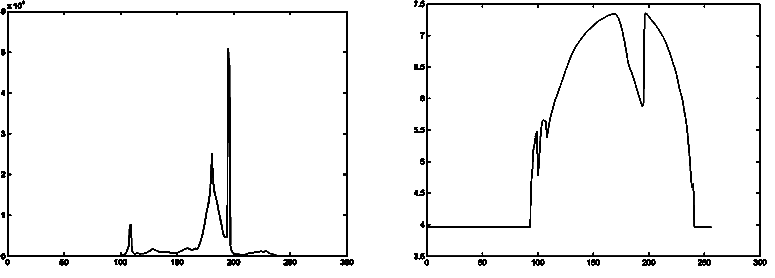
\includegraphics[scale=0.8]{Entropia.png}
	\caption{Porównanie histogramu i funkcji entropii. Źródło: \cite{2}}
	\label{fig:entr_hist}
\end{figure}

\section{Wyznaczanie obszaru zainteresowania}
Pomimo występowania rożnorodnych pasów ruchu w rzeczywistości, część ich cech charakterystycznych pozostaje bez zmian.
W wyniku zjawiska perspektywy, czym obiekt jest dalej od kamery tym staje się mniejszy, linie drogowe bliżej kamery, w dolnej części obrazka, są grubsze od tych znajdujących się dalej, w wyższej części obrazu.
To samo dotyczy całego pasa ruchu. W~dolnym obszarze obrazu występuje większy stosunek obiektu pierwszoplanowego, którym jest pas ruchu w~stosunku do~tła, reprezentowanego przez pobocze i obszar poza drogą.
Dodatkowo linie znajdujące się bliżej kamery wakazują na obrazie mniejszą tendencję do nagłej zmiany swojego położenia.
Natomiast nawet lekkie zakręty powodują nagłe przesunięcia się obiektów w~górnej części obrazu.
Podane zależności są charakterystyczne dla obrazów przedstawiających fragment ulicy wzdłuż której porusza się samochód.
Przyczyniło się to powstanie różnych konceptów wyznaczania ROI (ang. \textit{Region Of Interest} -- obszar zainteresowania).
W~pracach \cite{2} i~\cite{4} wykorzystano określenie statycznego obszaru zainteresowania.
ROI jest w kształcie trapezu zwężającego się w kierunku górnej części obrazu \cite{4}.

Wyznaczanie obszaru zainteresowania na obrazie może odbywać w sposób statyczny albo dynamiczny. 
Wyznaczanie statyczne polega na predefiniowanych ograniczeniach, na podstawie których otrzymywany jest obraz przetworzony. 
Dynamiczne odnosi się do sytuacji, w~której wyznaczony obszar zainteresowania zależny jest od danych wejściowych. 
W artykule \cite{vanishing_point} przedstawiono podejście polegające na wyznaczaniu obszaru zainteresowania na podstawie określonego punktu na horyzoncie.
Jest to punkt przecięcia się dwóch prostych, powstałych w skutek przedłużenia linii określających krawędzie drogi. 
Celem wyznaczenia ROI jest pozbycie się jak największej części obrazu, na której nie znajduje się pas ruchu.
Ma to na celu zmniejszenie wpływu tła na działanie algorytmów do detekcji linii.

\section{Wyznaczanie linii drogowych}
W tym etapie skupimy się na detekcji pasów ruchu poprzez wyznaczenie linii na~podstawie obrazu binarnego. 
W~artykule \cite{reichenbach_comparison} wykorzystano w tym celu transformatę Hough'a. 
Jest to metoda wykrywania prostych w~widzeniu komputerowym \cite{hough}.

Prostą znajdującą się na obrazie o współrzędnych kartezjańskich ${x,y}$ można zapisać jako punkt w układzie o współrzędnych $\theta$, $\rho$ \ref{fig:rotheta} (przestrzeń Hough'a) spełniający zależność \eqref{eq:2}, gdzie $\theta$ - kąt nachylenia, $\rho$ - odległość od początku układu współrzędnych.

\begin{equation}
\,x\cos(\theta )+\,y\sin(\theta )=\rho \label{eq:2}
\end{equation}


W celu wyznaczenia pełnego obrazu w przestrzeni Hough'a należy przeiterować po całym przetwarzanym obrazie i dla każdego piksela o wartości 1 (białego) zaznaczyć w układzie $\theta$, $\rho$ wszystkie punkty odpowiadające prostym we współrzędnych ${x,y}$ jakie mogą przechodzić przez ten piksel.

\begin{figure}
	\centering
	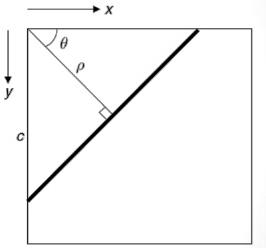
\includegraphics[scale=0.8]{hough_rotheta.png}
	\caption{Graficzne przedstawienie zależności współrzędnych ${x,y}$ i $\theta$, $\rho$. Źródło: \cite{hough_rotheta}}
	\label{fig:rotheta}
\end{figure}

Zakres grubości pasów znajdujących się przykładowo na autostradzie jest ściśle określony przepisami ruchu drogowego. 
Ta zależność została wykorzystana w pracy \cite{4}, gdzie użyto filtru wykrywającego linie ruchu drogowego. Działa on na zasadzie sprawdzania odległości w~poziomie pomiędzy dwoma białymi pikselami. Jeśli mieści się on w ustalonej normie oznacza to, że punkty leżą na linii.
Zakres dobierany jest w~zależności od badanej części obrazu, z zachowaniem właściwości perspektywy \ref{fig:lmps_sobe}. 



\begin{figure}
	\centering
	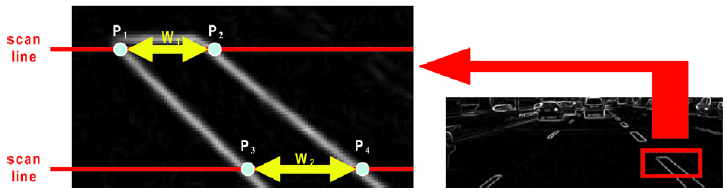
\includegraphics[scale=0.6]{lmps_sobe.png}
	\caption{Zdjęcie przedstawiająca sprawdzanie odległości w poziomie pomiędzy dwoma białymi pikselami. Źródło: \cite{4}}
	\label{fig:lmps_sobe}
\end{figure}

\section{Fuzja obrazu oraz~danych z~mapy}

Postrzeganie otoczenia jest jednym z~głównych wyzwań dla systemów w~pojazdach autonomicznych. 

Przednia kamera w~pojeździe dostarcza informacji o~kluczowych elementach drogi takich jak oznaczenia pasa ruchu i~jego granice. 
Poprawna detekcja przestrzeni, po której auto może się poruszać jest poważnym wyzwaniem ze względu na występowanie wielu pasów ruchu, przecinania się linii.

W artykule \cite{hdmap} podjęto się przeprowadzenia fuzji detekcji pasa ruchu drogowego oraz informacji z~HD (ang. \textit{High Definition} -- wysoka rozdzielczość) mapy. 
Informacja o obecnym położeniu auta zapewniła możliwość wyekstrahowania z~mapy danych o~kształcie drogi na jakiej się znajdował.

Zaproponowane podejście ma znaczącą przewagę nad korzystaniem z~samej kamery, ponieważ jest w~stanie rekompensować skutki takich błędów jak: 
\begin{enumerate}
	\item zmienne warunki oświetlenia, obraz może zawierać nieregularne cienie lub przebłyski,
	\item brak widoczności linii drogowych, naruszona tekstura krawędzi,
	\item nieregularna kolorystycznie nawierzchnia drogowa lub  obiekty ją przysłaniające,
	\item kamera może nie uchwycić całego obszaru, który powinien zostać wykryty, ze względu na krzywiznę drogi.
\end{enumerate}
W~sytuacji, gdy z~obrazu nie da się uzyskać wystarczających informacji przykładowo o~nagłym zakręcie na drodze, dane z~mapy mogą okazać się nieocenione.

\chapter{Opis platformy sprzętowej}

\section{Specyfikacja sprzętowa platformy Zybo}

\begin{figure}[h]
	\centering
	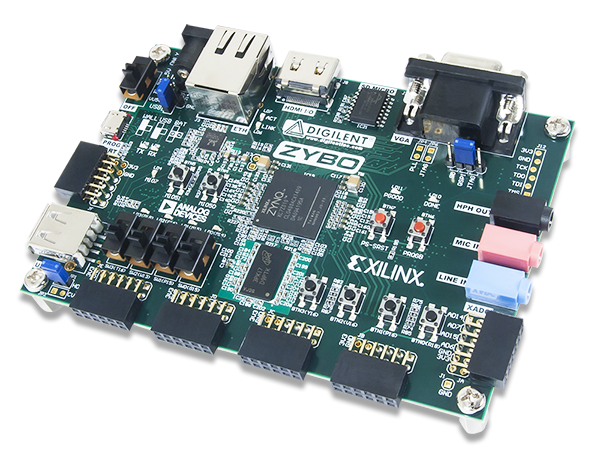
\includegraphics[scale=2]{zybo_img.png}
	\caption{Platforma Zybo z~układem Zynq SoC. Źródło: \cite{zybo_img}}
	\label{fig:zybo_img}
\end{figure}

Do implementacji sprzętowej została wykorzystana karta Zybo firmy Digilent \ref{fig:zybo_img} wyposażona w~układ Zynq SoC (ang. \textit{System on Chip}). 
W~dokumencie \cite{zybo_description} znajduje się opis budowy układu. 
Jest on określany mianem "heterogeniczny", ponieważ zawiera dwa rodzaje zasobów sprzętowych: dwurdzeniowy procesor ARM Cortex-A9 oraz układ FPGA(ang.\textit{Field Programmable Gate Array} -- bezpośrednio programowalna macierz bramek), czyli logikę reprogramowalną.

\subsection{Logika reprogramowalna}



Część reprogramowalna układu Zynq na karcie Zybo jest oparta o~logikę serii  Artix-7 firmy Xilinx. 
Podstawowym elementem z~którego zbudowane jest FPGA, to blok CLB (ang. \textit{Configurable Logic Block}). 
Składa się on z~dwóch Slice'ów połączonych z~matrycą przełączeń (ang. \textit{Switch Matrix}). 
W~układach Zynq występują dwa rodzaje elementów Slice, są to SliceL i SliceM. 
Slice typu M składa się z:
\begin{itemize}
	\item generatora funkcyjnego (4 sztuki) -- został on zrealizowany przy pomocy układów LUT (ang. \textit{Look-Up Table}). Posiada 6 wejść i~2 wyjścia. Może także zostać skonfigurowany jako synchroniczna pamięć RAM lub 32 bitowy rejestr przesuwny wykorzystywany w~liniach opóźniających,
	\item przerzutnika typu D (FF -- ang. \textit{Flip-Flop}) -- slice zawiera 8 sztuk, przy czym 4 mogą zostać skonfigurowane jako zatrzask (ang. \textit{latch}),
	\item multiplekserów,
	\item szybkiej logiki przeniesienia.
\end{itemize}

Do pozostałych zasobów dostępnych w układach FPGA serii Artix-7 należą:
\begin{itemize}
	\item CMT (ang. \textit{Clock Managment Tiles}) -- bloki umożliwiające zarządzanie sygnałem zegarowym, generowanie różnych częstotliwości zegara, równomierną propagację sygnału, tłumienie zjawiska zakłócenia fazy zegara,
	\item Block RAM (BRAM) -- blokowa dwuportowa pamięć RAM o~rozmiarze 36Kb (na blok). Może zostać skonfigurowana jako moduł FIFO (ang. \textit{First In First Out}),
	\item DSP48A1 -- moduł zawierający mnożarkę 25x18 bitów oraz akumulator 48 bitowy. Liczba modułów zależy od rozmiaru układu i~zawiera się w przedziale od 66 do 2020,
	\item Select I/O -- banki zasobów wejścia/wyjścia, których liczba zawiera się w~przedziale od 100 do 400 końcówek podłączonych do części FPGA, 
	\item GTP/GTX Transceivers -- moduły umożliwiające transmisję szeregową z~prędkością do 12,5 Gb/s (GTX) i~6,25 (GTP).
\end{itemize}

\subsection{System procesorowy}
ARM Cortex-A9 MPCore jest 32 bitowym procesorem firmy ARM Holdings z~zaimplementowaną archtekturą ARMv7-A. 
Zawiera od 1 do 4 rdzeni. 
Płytka Zybo Zynq SoC jest wyposażona w~wersje procesora dwurdzeniowego.
Rozkazy procesorów ARM są tak skonstruowane, aby wykonywały jedną określoną operację w~jednym cyklu maszynowym.
Kluczowymi cechami rdzenia Cortex-A9 są \cite{armCortex}:

\begin{itemize}
	\item NEON SIMD (ang. \textit{single instruction, multiple data} -- pojedyncza instrukcja, wiele danych) opcjonalne rozszerzenie zestawu instrukcji do 16 operacji na instrukcję,
	\item jednostka zmiennoprzecinkowa VFPv3 dwukrotnie przewyższająca wydajność swojego poprzednika ARM FPUs,
	\item kodowanie zestawu instrukcji Thumb-2 zmniejsza rozmiar programów, co poprawia wydajność,
	\item rozszerzenia zabezpieczeń TrustZone,
	\item program Trace Macrocell i~CoreSight Design Kit do nieinwazyjnego śledzenia wykonywania instrukcji,
	\item kontroler pamięci podręcznej L2 (0-4 MB),
	\item przetwarzanie wielordzeniowe,
	\item kontroler pamięci statycznej, dynamicznej i bezpośredniej.
\end{itemize}

\chapter{Implementacja modelu programowego}

W celu przetestowania wybranych algorytmów zdecydowano się wykorzystać tzw. model programowy tworzonej aplikacji. 
Do zaimplementowania prototypu wybrano komputer z~procesorem Intel Core i7 6700HQ. 
Posłużono się językami programowania Matlab.
Z racji tego, że algorytmy miały zostać zaimplementowane z~myślą o~późniejszych przeniesieniu ich na część reprogramowalną platformy Zynq SoC.
%Język Python okazał się niewystarczającym narzędziem z~racji tego, że algorytmy miały zostać zaimplementowane z~myślą o~późniejszych przeniesieniu ich na część reprogramowalną platformy Zynq SoC. 
Na jeden takt zegara otrzymuje się jeden piksel (co wynika ze sposobu obsługi sygnału wideo).
Z każdym kolejnym taktem otrzymuje się kolejne piksele. W~celu przeprowadzenie operacji kontekstowych należy korzystając z~linii opóźniających zrobić tak, aby w~danym takcie zegara mieć dostęp do wszystkich pikseli tworzących kontekst. Takie podejście powoduje, że niektóre algorytmy nie są możliwe do zaimplementowania. Należy zrezygnować ze wszystkich algorytmów, w których każdy kolejny krok algorytmu jest zależny od danych wejściowych, np. segmentacja przez rozrost. %Model programowy zbudowano tak, że w~jednej iteracji otrzymywano dostęp do jednego piksela. Taka funkcjonalność zaimplementowana w języku Python wprowadza bardzo duże opóźnienia. Jest to spowodowane faktem, że w~tym języku tabela elementów reprezentowana jest jako tabela wskaźników, gdzie każdy wskaźnik odnosi się do odpowiedniego miejsca w~pamięci. %Język Cython jest połączeniem języka Python oraz C. W~tym języku istnieje możliwość stworzenia tabeli, do której obsługi wystarczy jeden wskaźnik. Wszystkie elementy tabeli zapisane są w~pamięci komputera w~sposób uporządkowany. Odwołując się do kolejnych wartości tabeli wykorzystuje się tylko jeden wskaźnik. Powoduje to znacznie szybsze wykonanie iteracji po obrazie. Dlatego też funkcje przetwarzające obraz zdecydowano się napisać w~języku Cython. Plik główny, w~którym wykonywane są wspomniane funkcje napisany został w języku Python.% Do wczytania pliku wideo wykorzystano bibliotekę OpenCV.

Aplikacja ma na celu detekcję punktów reprezentujących prawą i lewą linie drogową. %W implementacji programowej zdecydowano się wykorzystać bibliotekę OpenCV do aproksymacji wielomianowej wyznaczonych punktów.
\chapter{Implementacja sprzętowa}

\section{Binaryzacja}

W celu ekstrakcji obrazu zbinaryzowanego z~obrazu w~formacie RGB zdecydowano się wykorzystać binaryzację ze stałym progiem. 
Obraz wejściowy najpierw konwertowany jest do obrazu w~odcieniach szarości. 
W~formacie RGB na każdy piksel składają się trzy kanały, każdy o~wartości z~przedziału 0-255 zapisane na 8 bitach. 
Największe i najmniejsze wartości z~kanałów są dodawane i~dzielone przez 2. 
Operacja ta zostaje przeprowadzona dla każdego piksela.
Zdecydowano się na taką metodę, ponieważ dzielenie przez liczbę, która jest wielokrotnością 2 może zostać zrealizowane poprzez przesunięcie bitowe. Jest ono znacznie szybsze niż użycie dzielarki. W porównaniu do wyliczania średniej z trzech kanałów, zachowujemy pełny zakres od 0 do 255 i nie musimy wykorzystywać dzielarki.
Obrazem wynikowym jest obraz w~odcieniach szarości, który kolejno jest poddawany binaryzacji.

\noindent Rysunki \ref{fig:in_otsu_fpga}, \ref{fig:out_otsu_fpga} przedstawiają efekt symulacji tego algorytmu dla obrazu o~wymiarach 348x128. 

\begin{figure}[h]
		\centering
		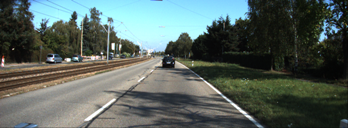
\includegraphics[scale=0.8]{obraz_color_smal.png}
		\caption{Obraz wejściowy do symulacji sprzętowej binaryzacji}
		\label{fig:in_otsu_fpga}
\end{figure}

\begin{figure}[h]
		\centering
		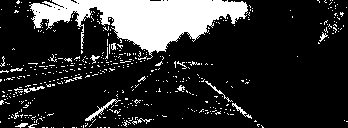
\includegraphics[scale=0.8]{obraz_bin_smal.png}
		\caption{Obraz wyjściowy z symulacji sprzętowej binaryzacji}
		\label{fig:out_otsu_fpga}
\end{figure}

\section{Wyznaczanie ROI}
Efekty symulacji implementacji sprzętowej wyznaczania obszaru zainteresowania zostały przedstawione na rysunku \ref{fig:roi_sym}.


Opis schematu \ref{fig:roi_symmm} implementacji sprzętowej algorytmu do wyznaczenia współczynników wykorzystywanych w \ref{fig:roi_symm2}(w nawiasach podano liczbę bitów potrzebną do zapisania danej wartości albo liczbę taktów zegara potrzebnych do przeprowadzania danej operacji):
\begin{itemize}
	\item A - współrzędna x piksela, poz\_x (12 bity),
	\item B - stała wartość równa 3 (4 bity),
	\item C - jedna ósma szerokości obrazu (12 bitów),
	\item D - stała wartość równa 5 (4 bity),
	\item W1 - współczynnik 1 (16 bitów),
	\item W2 - współczynnik 2 (16 bitów),
	\item (-) - odejmowanie (1 takt zegara),
\end{itemize}
Rezultaty odejmowania W1 i W2 są kolejno wykorzystywane w logice asynchronicznej \ref{fig:roi_symm2}
\begin{figure}[h]
	\centering
	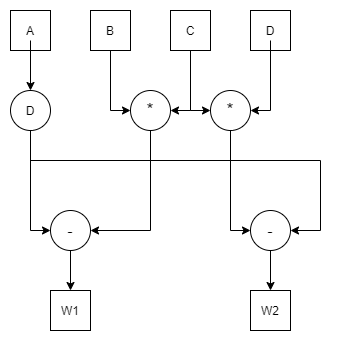
\includegraphics[scale=0.5]{ROI_schem.png}
	\caption{Schemat algorytmu do wyznaczania współczynników dla ROI.}
	\label{fig:roi_symmm}
\end{figure}
\begin{figure}[h]
	\centering
	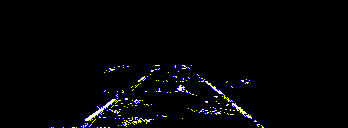
\includegraphics[scale=0.8]{obraz_roi_smal.png}
	\caption{Obraz wyjściowy z symulacji sprzętowej algorytmu do wyznaczania ROI.}
	\label{fig:roi_sym}
\end{figure}

\begin{figure}[h]
	\centering
	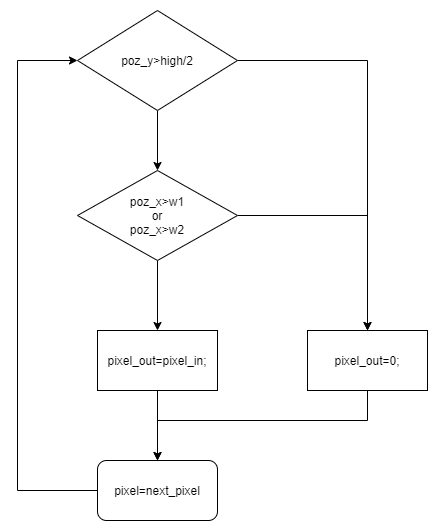
\includegraphics[scale=0.5]{ROI_blockowy.png}
	\caption{Schemat algorytmu do wyznaczania ROI. Wartości współczynnik1 i współczynnik2 są rezultatami \ref{fig:roi_symmm}}
	\label{fig:roi_symm2}
\end{figure}
\section{LMPS}

\begin{figure}[h]
	\centering
	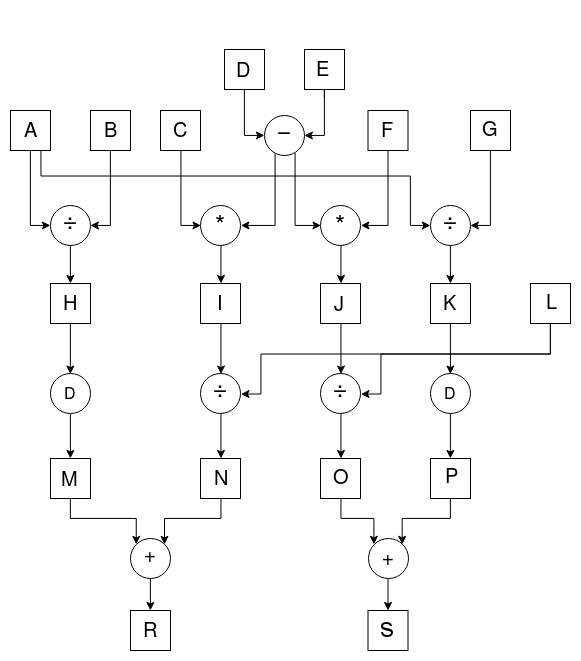
\includegraphics[scale=0.4]{impl_dev_lmps_1.png}
	\caption{Schemat blokowy implementacji sprzętowej algorytmu do wyznaczenia ograniczeń górnych i dolnych dla filtru LMPS}
	\label{fig:lmps1}
\end{figure}

Opis schematu implementacji sprzętowej algorytmu do wyznaczenia ograniczeń górnych i~dolnych \ref{fig:lmps1}:
\begin{itemize}
	\item A - szerokość obrazu (32 bity),
	\item B - stała zależna od grubości linii drogowych, wynosi 400 (20 bitów),
	\item C - stała zależna od grubości linii drogowych, wynosi 20 (8 bitów),
	\item D - indeks wiersza obecnego piksela (24 bity),
	\item E - połowa szerokości obrazu (24 bity),
	\item F - stała zależna od grubości linii drogowych, wynosi 62 (8bitów),
	\item G - stała zależna od grubości linii drogowych, wynosi 90 (20 bitów),
	\item L - wysokość obrazu (20 bitów),
	\item H, K, N, O - rezultaty dzielenia (32 bity),
	\item I, J - rezultaty mnożenia (32 bity),
	\item M, P - sygnały wyjściowe z linii opóźniających (32 bity),
	\item R - próg ograniczający dolny (32 bity),
	\item S - próg ograniczający górny (32 bity),
	\item ($\div$) - dzielenie (4 takty zegara),
	\item (*) - mnożenie (1 takt zegara),
	\item (D) - linia opóźniająca (1 takt zegara),
	\item (+) - dodawanie (1 takt zegara).
	\item (-) - odejmowanie (1 takt zegara).
\end{itemize}
Progi ograniczające dolny i~górny wykorzystywane są kolejno w~logice asynchronicznej przedstawionej na schemacie \ref{fig:lmps2}. 
Nie zamieszczono rysunków z~symulacji implementacji sprzętowej, ponieważ dla obrazów o~rozmiarze tak małym jak 348x128, filtr nie daje rzetelnych rezultatów. 
W~modelu programowym wykorzystano obraz o~rozmiarze 1392x512. 
Tak znaczne zmniejszenie go oraz zniekształcenie powoduje zaburzenie działania filtru. 
Wynika to z~tego, że działanie filtru jest zależne od wysokości i~szerokości obrazu.

\begin{figure}[!]
	\centering
	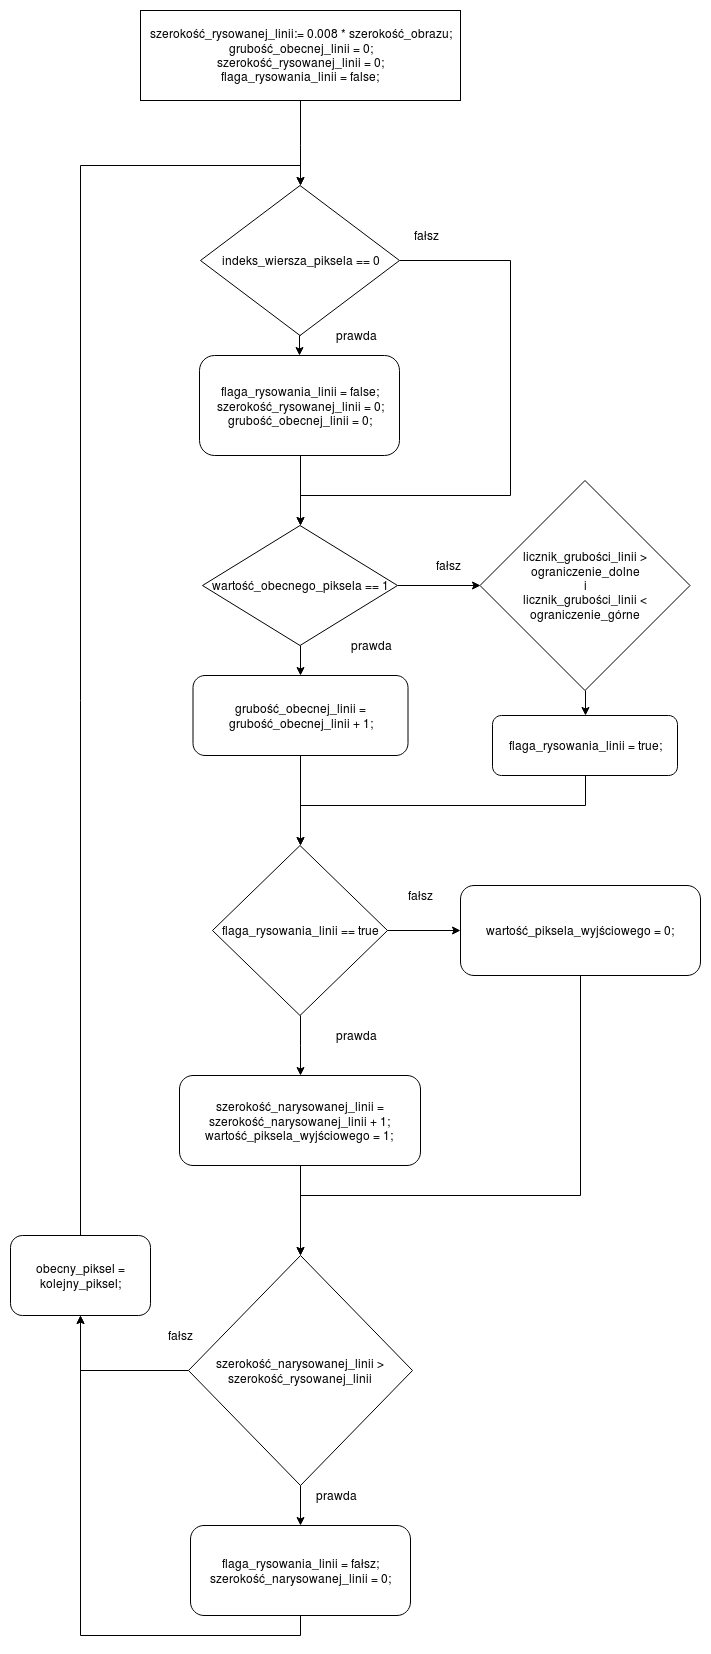
\includegraphics[scale=0.35]{impl_dev_lmps_2.png}
	\caption{Schemat blokowy implementacji sprzętowej algorytmu do odfiltrowania elementów nie będących liniami ruchu drogowego.}
	\label{fig:lmps2}
\end{figure}


\section{Podział obrazu}

W celu wyznaczenia środków ciężkości w określonych strefach na obrazie, wykorzystuje się implementacje sprzętową(dla każdego obszaru oddzielnie) przedstawioną na schemacie \ref{fig:wyzn_sc}. Jeśli, któryś z liczników po przeiterowaniu całego obrazu jest równy 0, środek nie jest wyznaczany.
\begin{figure}[h]
	\centering
	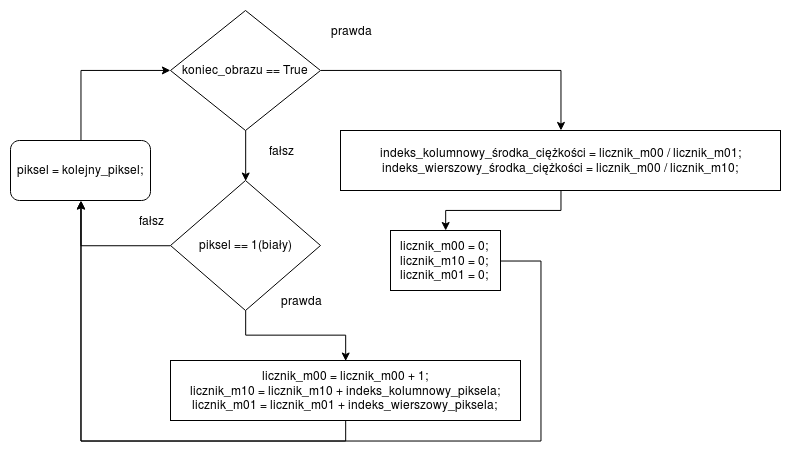
\includegraphics[scale=0.6]{wyzn_sc.png}
	\caption{Schemat blokowy implementacji sprzętowej algorytmu do wyznaczenia środka ciężkości.}
	\label{fig:wyzn_sc}
\end{figure}
\chapter{Testy}

Zaimplementowane algorytmy przetestowano na materiałach pobranych z internetu \cite{Geiger2013IJRR}.
Na~zdjęciu \ref{fig:mod_img_test1} przedstawiono obraz oryginalny z~naniesionymi niebieską i~zieloną krzywą, które powstały w~wyniku aproksymacji wielomianowej środków ciężkości (czerwone punkty).
Na~zdjęciu \ref{fig:mod_img_test1_bin} przedstawiono efekt binaryzacji, a~na~zdjęciu \ref{fig:mod_img_test1_roi} już po wyznaczeniu ROI. Na~obrazie \ref{fig:mod_img_test1_lmps} po~zastosowaniu filtru LMPS. W~tym wypadku detekcja linii przebiegła bez żadnych problemów.

W~sytuacji, gdy na drogę pada zbyt mocne światło i odbija się od niej, tak jak zostało przed stawione na zdjęciach \ref{fig:mod_img_test2}, \ref{fig:mod_img_test3} i \ref{fig:mod_img_test4}, detekcji linii napotykał nie była już tak poprawna jak przy jednolitym oświetleniu.
Na obrazku \ref{fig:mod_img_test2}, można zauważyć, że~pomimo pewnych błędów otrzymana krzywa jest wględnie pokrywająca się z  pasami ruchu. Natomiast na obrazku \ref{fig:mod_img_test3} pomimo refleksów udało się poprawnie wykryć lewy pas ruchu drogowego.
Najgorzej przebiegła detekcja linii na obrazku \ref{fig:mod_img_test4}, gdzie filtracja LMPS najgorzej poradziła sobie z odfiltrowaniem zakłóceń wynikających z refleksów świetlnych.

W przypadku zdjęcia \ref{fig:mod_img_test5} mamy do czynienia z mocno zacienionym prawym pasem ruchu oraz fragment jezdni z skośnymi pasami z lewej. W wyniku bardzo jasnej scenerii zdjęcia, pas znajdujący się w cieniu jest ciemniejszy niż zakładany próg binaryzacji w wyniku czego, nie został on poprawnie wykryty. Dodatkowo filtr LMPS nie poradził sobie w pełni poprawnie z odfiltrowaniem skośnych pasów, co zaburzyło późniejsze obliczanie środków ciężkości.

Algorytm nie ma problemów z detekcją jezdni w przypadku prostej drogi i dobrych warunków oświetleniowych.
wyzwanie pojawia się przy nie jednolitym oświetleniu, gdyż albo część obiektów zlewa się w refleksach świetlnych, albo zostaje ukrytych w cieniu, co znacząco utrudnia późniejszą detekcję linii pasa ruchu drogowego przez filtr LMPS.

\begin{figure}[h]
	\begin{minipage}{0.48\textwidth}
		\centering
		\includegraphics[scale=0.20]{test1_color_linie.png}
		\caption{Obraz prostej drogi z naniesionymi środkami ciężkości oraz wykrytymi liniami.}
		\label{fig:mod_img_test1}
	\end{minipage}
	\begin{minipage}{0.48\textwidth}
		\centering
		\includegraphics[scale=0.15]{test1_bin.png}
		\caption{Obraz \ref{fig:mod_img_test1} po zbinaryzowaniu.}
		\label{fig:mod_img_test1_bin}
	\end{minipage}
\end{figure}

\begin{figure}[h]
	\begin{minipage}{0.48\textwidth}
		\centering
		\includegraphics[scale=0.15]{test1_roi.png}
		\caption{Obraz \ref{fig:mod_img_test1_bin} po wyznaczeniu ROI.}
		\label{fig:mod_img_test1_roi}
	\end{minipage}
	\begin{minipage}{0.48\textwidth}
		\centering
		\includegraphics[scale=0.15]{test1_lmps.png}
		\caption{Obraz \ref{fig:mod_img_test1_roi} po zastosowaniu filtru LMPS.}
		\label{fig:mod_img_test1_lmps}
	\end{minipage}
\end{figure}



\begin{figure}
	\begin{minipage}{0.48\textwidth}
		\centering
		\includegraphics[scale=0.20]{test2_color_linie.png}
		\caption{Obraz prostej drogi z refleksami wraz z naniesionymi środkami ciężkości oraz wykrytymi liniami.}
		\label{fig:mod_img_test2}
	\end{minipage}
	\begin{minipage}{0.48\textwidth}
		\centering
		\includegraphics[scale=0.15]{test2_bin.png}
		\caption{Obraz \ref{fig:mod_img_test2} po zbinaryzowaniu.}
		\label{fig:mod_img_test2_bin}
	\end{minipage}
\end{figure}

\begin{figure}
	\begin{minipage}{0.48\textwidth}
		\centering
		\includegraphics[scale=0.15]{test2_roi.png}
		\caption{Obraz \ref{fig:mod_img_test2_bin} po wyznaczeniu ROI.}
		\label{fig:mod_img_test2_roi}
	\end{minipage}
	\begin{minipage}{0.48\textwidth}
		\centering
		\includegraphics[scale=0.15]{test2_lmps.png}
		\caption{Obraz \ref{fig:mod_img_test2_roi} po zastosowaniu filtru LMPS.}
		\label{fig:mod_img_test2_lmps}
	\end{minipage}
\end{figure}




\begin{figure}
	\begin{minipage}{0.48\textwidth}
		\centering
		\includegraphics[scale=0.20]{test3_color_linie.png}
		\caption{Obraz prostej drogi z refleksami wraz z naniesionymi środkami ciężkości oraz wykrytymi liniami.}
		\label{fig:mod_img_test3}
	\end{minipage}
	\begin{minipage}{0.48\textwidth}
		\centering
		\includegraphics[scale=0.15]{test3_bin.png}
		\caption{Obraz \ref{fig:mod_img_test3} po zbinaryzowaniu.}
		\label{fig:mod_img_test3_bin}
	\end{minipage}
\end{figure}

\begin{figure}
	\begin{minipage}{0.48\textwidth}
		\centering
		\includegraphics[scale=0.15]{test3_roi.png}
		\caption{Obraz \ref{fig:mod_img_test3_bin} po wyznaczeniu ROI.}
		\label{fig:mod_img_test3_roi}
	\end{minipage}
	\begin{minipage}{0.48\textwidth}
		\centering
		\includegraphics[scale=0.15]{test3_lmps.png}
		\caption{Obraz \ref{fig:mod_img_test3_roi} po zastosowaniu filtru LMPS.}
		\label{fig:mod_img_test3_lmps}
	\end{minipage}
\end{figure}



\begin{figure}
	\begin{minipage}{0.48\textwidth}
		\centering
		\includegraphics[scale=0.20]{test4_color_linie.png}
		\caption{Obraz prostej drogi z refleksami wraz z naniesionymi środkami ciężkości oraz wykrytymi liniami.}
		\label{fig:mod_img_test4}
	\end{minipage}
	\begin{minipage}{0.48\textwidth}
		\centering
		\includegraphics[scale=0.15]{test4_bin.png}
		\caption{Obraz \ref{fig:mod_img_test4} po zbinaryzowaniu.}
		\label{fig:mod_img_test4_bin}
	\end{minipage}
\end{figure}

\begin{figure}
	\begin{minipage}{0.48\textwidth}
		\centering
		\includegraphics[scale=0.15]{test4_roi.png}
		\caption{Obraz \ref{fig:mod_img_test4_bin} po wyznaczeniu ROI.}
		\label{fig:mod_img_test4_roi}
	\end{minipage}
	\begin{minipage}{0.48\textwidth}
		\centering
		\includegraphics[scale=0.15]{test4_lmps.png}
		\caption{Obraz \ref{fig:mod_img_test4_roi} po zastosowaniu filtru LMPS.}
		\label{fig:mod_img_test4_lmps}
	\end{minipage}
\end{figure}



\begin{figure}
	\begin{minipage}{0.48\textwidth}
		\centering
		\includegraphics[scale=0.20]{test5_color_linie.png}
		\caption{Obraz prostej drogi z mocno zacienionym pasem ruchu, wraz z naniesionymi środkami ciężkości oraz wykrytymi liniami.}
		\label{fig:mod_img_test5}
	\end{minipage}
	\begin{minipage}{0.48\textwidth}
		\centering
		\includegraphics[scale=0.15]{test5_bin.png}
		\caption{Obraz \ref{fig:mod_img_test5} po zbinaryzowaniu.}
		\label{fig:mod_img_test5_bin}
	\end{minipage}
\end{figure}

\begin{figure}
	\begin{minipage}{0.48\textwidth}
		\centering
		\includegraphics[scale=0.15]{test5_roi.png}
		\caption{Obraz \ref{fig:mod_img_test5_bin} po wyznaczeniu ROI.}
		\label{fig:mod_img_test5_roi}
	\end{minipage}
	\begin{minipage}{0.48\textwidth}
		\centering
		\includegraphics[scale=0.15]{test5_lmps.png}
		\caption{Obraz \ref{fig:mod_img_test5_roi} po zastosowaniu filtru LMPS.}
		\label{fig:mod_img_test5_lmps}
	\end{minipage}
\end{figure}

Dodatkowo w celu przetestowania algorytmu w przypadku zmiany pasa ruchu i przypadku z pasami w kolorze żółtym posłużyłem się nagraniem jazdy po autostradzie, z przedniej kamery samochodowej, pobranym z internetu \cite{youtube_mat}.
Na zdjęciu \ref{fig:mod_img_test6} przedstawiono wynik poprawnej detekcji pasów podczas jazdy prosto.
Podczas manewru zmiany pasa ruchu \ref{fig:mod_img_test6_a}, \ref{fig:mod_img_test6_b} lewa linia pasa ruchu przestaje być wykrywana. Jest to spowodowane wyznaczaniem ROI, gdyż linia zostaje przesuniętą po za obszar detekcji. Natomiast prawa linia jest wykrywa bez zarzutów.
Na zdjęciu \ref{fig:mod_img_test6_c} przedstawiono rezultat wykorzystanych algorytmów, w~sytuacji gdy prawa linia  drogowa ma kolor żółty, a lewa dalej biały.
Detakcja przebiegła poprawnie dla obu przypadków. Z czego nawet lepiej dla linii żółtej, wykryto więcej środków ciężkości, co może być spowodowane mniejszymi odstępami pomiędzy linia pasa ruchu.

\begin{figure}
	\begin{minipage}{0.48\textwidth}
		\centering
		\includegraphics[scale=0.3]{test_prosta.png}
		\caption{Detekcja na prostej drodze na autostradzie.}
		\label{fig:mod_img_test6}
	\end{minipage}
	\begin{minipage}{0.48\textwidth}
		\centering
		\includegraphics[scale=0.3]{test_zmiana_pasa.png}
		\caption{Początek manewru zmiana pasa ruchu.}
		\label{fig:mod_img_test6_a}
	\end{minipage}
\end{figure}
\begin{figure}
	\begin{minipage}{0.48\textwidth}
		\centering
		\includegraphics[scale=0.3]{test_srodek_zmiany_pasa.png}
		\caption{Kontyunacja manewru wyprzedzania.}
		\label{fig:mod_img_test6_b}
	\end{minipage}
	\begin{minipage}{0.48\textwidth}
		\centering
		\includegraphics[scale=0.3]{test_zolty_pas.png}
		\caption{Detekcja linii z białymi i żółtymi pasamai.}
		\label{fig:mod_img_test6_c}
	\end{minipage}
\end{figure}

\chapter{Podsumowanie}

\section{Wnioski}
W ramach pracy inżynierksiej udało się zaimplementować model programowy w języku Matlab. 
Algorytm charakteryzował się jednak zauważalnym czasem obliczeń. Implementacje sprzętowe binaryzacji oraz wyznaczania obszaru zainteresowanie ROI udało się przetestować symulacyjnie. Porównanie wyników z implementacją programową świadczy o tym, że algorytmy zostały poprawnie zaimplementowane.
Symulacja możliwa była do przeprowadzanie dla obrazów o wymiarach 348x128. Dlatego też nie udało się przeprowadzić symulacji filtru LMPS. Znaczne zmniejsze i zniekształcenie względem orginalnego obrazu powoduje, że filtr nie daje rzetelnych rezultatów. Zamieszczone testy przeprowadzono na modelu programowym.
Przedstawionego podejscia nie udało się zaimplementować na platformie Zybo Zynq SoC ze względu na zdarzenia losowe.


\printbibliography
Do niniejszej pracy załączono płytę CD, na której znajduje się:
\begin{itemize}
	\item tekst pracy zapisany w formacie PDF i źródła Latex,
	\item kod źródłowy analizowanych algorytmów oraz środowiska testowego,
	\item dane wejściowe, na których przeprowadzane były testy porównawcze
\end{itemize}


% itd.
% \appendix
% \include{dodatekA}
% \include{dodatekB}
% itd.
%\printbibliography

\end{document}
